\section{Creating the Computational Domain}
%
\subsection{What you will Learn (Geom and Smesh)}
In this part, you will learn how to create the computational domain using the \geom and \smesh modules of \salome. Thanks to primitives available in \geom, creating the CAD will be easy and the work will essentially be in \smesh.
%
\subsection{Creating the CAD}
%
Once the files structure is created by following the step in \ref{lag:create_CS_struct}, move to the \geom module in \salome. We want to create two cylinders which will subsequently define two zones in the flow domain, upstream and downstream of the injection plane, respectively. The reason for creating two cylinders is that the mesh upstream of the injection point will be coarser than that downstream of it.  This will not have an impact on solution accuracy but will reduce the overall computational time. In the present part, a disk is created. In the following parts, it will be meshed and finally extruded to generate the two cylinders.

Create a Divided Disk by selecting \menu{New Entity > Blocks > Divided Disk}. This represents the inlet boundary:
%
\begin{itemize}
	\item \textbf{name:} inlet\_disk 
	\item  \textbf{Radius:} 0.045
	\item \textbf{Orientation:} OXY
	\item \textbf{Division pattern:} Hexagon
\end{itemize} 
%
\begin{figure}[hbtp]
	\centering
	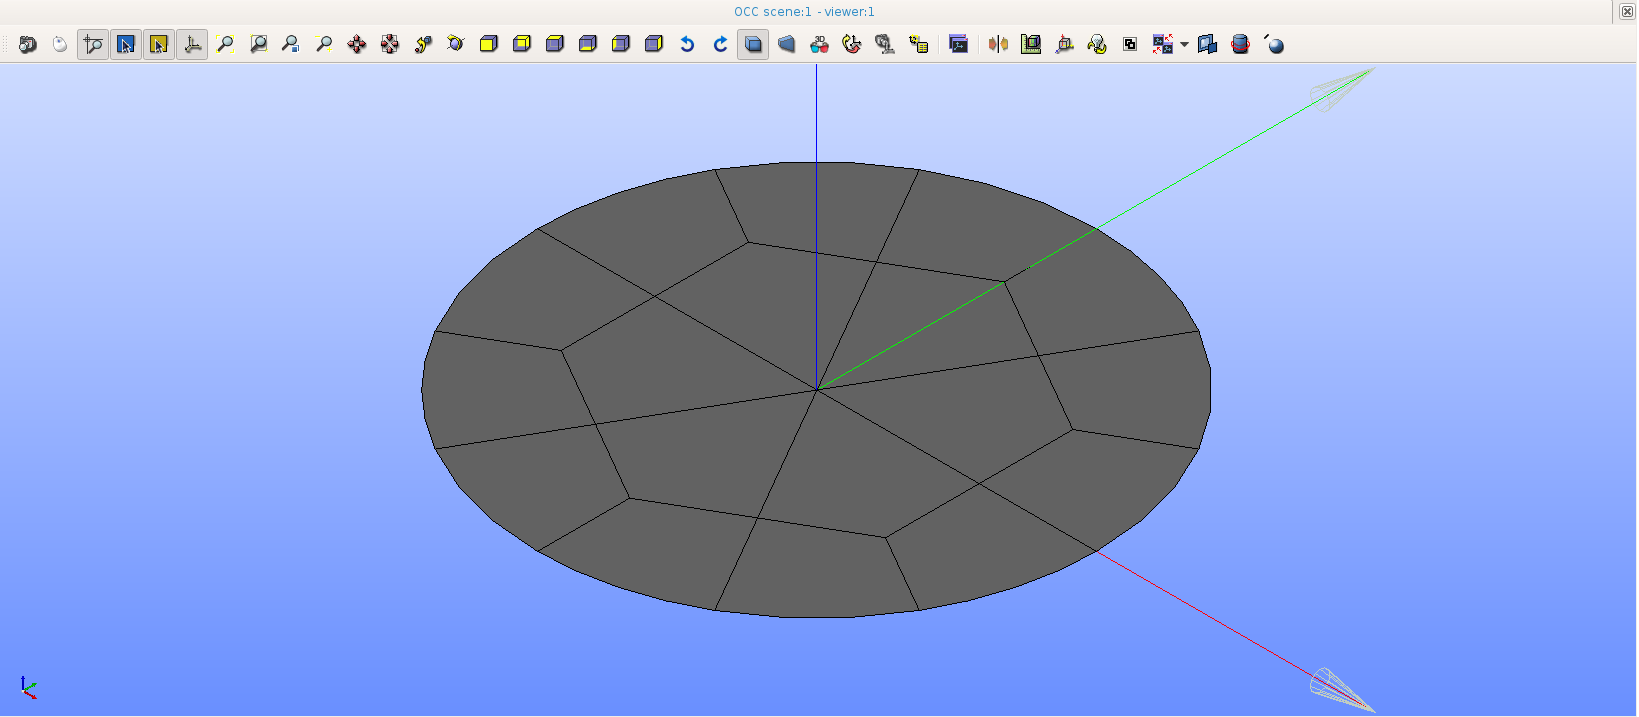
\includegraphics[width=0.8\textwidth]{\IMAGES/scdcylinder.png}
	\caption{Divided disk}
	\label{lag:scd_cylinder}
\end{figure}
%

Finally, create the two following points:
\begin{itemize}
	\item \textbf{name:} z\_4.0
	\item  \textbf{Coordinates} x: 0; y: 0, z: 4.0
\end{itemize} 
%
\begin{itemize}
	\item \textbf{name:} z\_5.9
	\item  \textbf{Coordinates} x: 0; y: 0, z: 5.9
\end{itemize} 
%
and the two following lines:
\begin{itemize}
	\item \textbf{name:} 0\_to\_4.0
	\item \textbf{Point 1:} O (origin, clic on O in Object Browser)
	\item \textbf{Point 2:} z\_4.0
\end{itemize} 
%
\begin{itemize}
	\item \textbf{name:} 4.0\_to\_5.9
	\item \textbf{Point 1:} z\_4.0 
	\item \textbf{Point 2:} z\_5.9
\end{itemize} 
%
\subsection{Creating Groups on \geom}
%
The next step is
to create some groups that will be used as boundary conditions by the numerical model.

Right click on inlet\_disk and select \textbf{Create Group}.
Select the edges composing the border of the disk and add them to the group (\figurename~\ref{lag:wall_group}). It will be our boundary condition "wall".
%
\begin{itemize}
	\item \textbf{Shape Type:} edges
	\item \textbf{Group Name:} wall
	\item \textbf{Main Shape:} inlet\_disk
	\item \textbf{Main Shape Selection restriction}: No restriction
\end{itemize}
%
\begin{figure}[H]
	\centering
	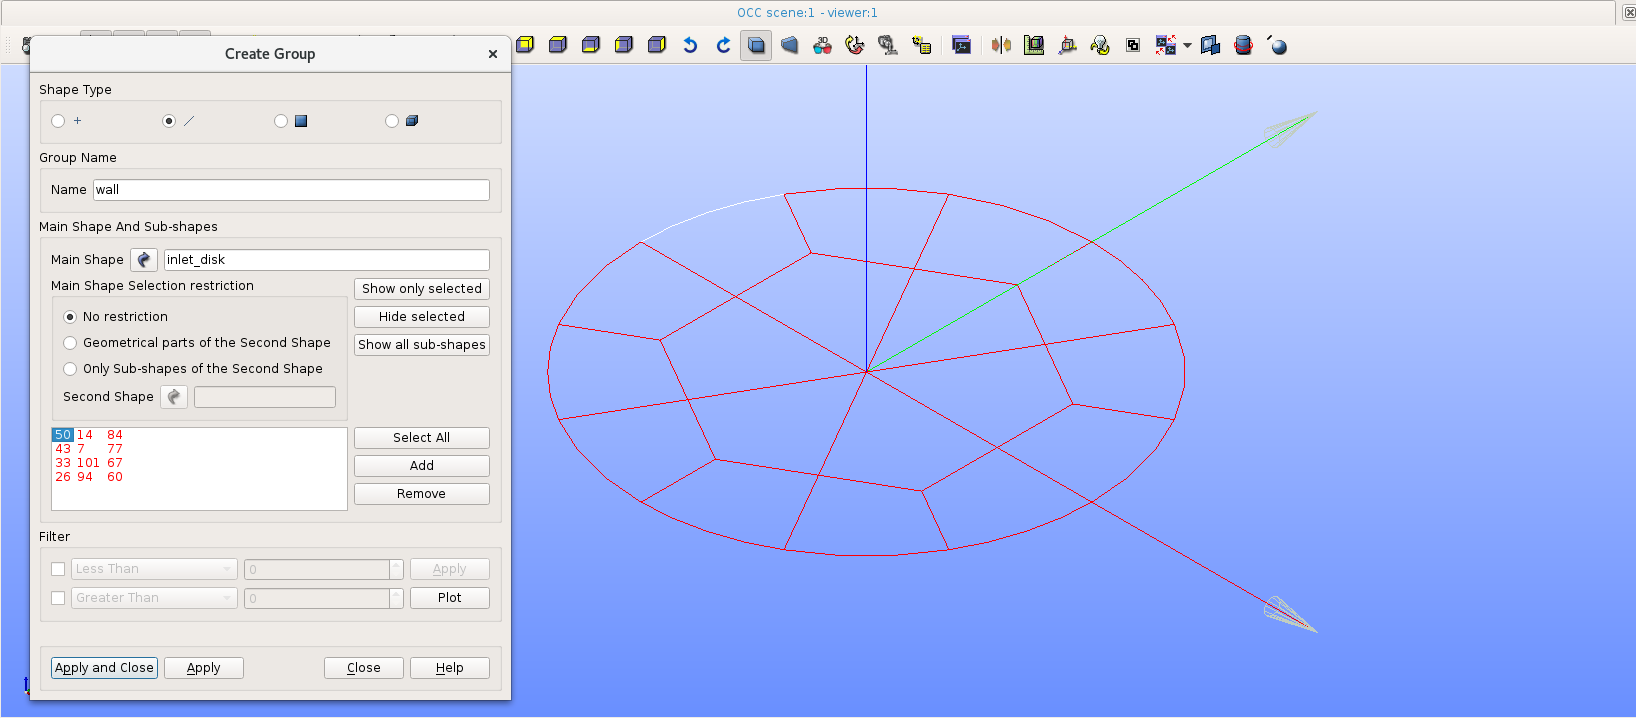
\includegraphics[width =\linewidth]{\IMAGES/wall_point.png}
	\caption{Creation of the group ``wall''}
	\label{lag:wall_group}
\end{figure}
%
\clearpage
%
\subsection{Meshing}
%
Move to the module 'Mesh' (\smesh) of \salome. Select inlet\_disk in the object browser and \menu{Mesh > Create Mesh}.
%
\begin{itemize}
	\item \textbf{Name:} inlet\_mesh
	\item \textbf{Geometry:} inlet\_disk
	\item \textbf{Mesh type:} Any
	\item \menu{2D > Algorithm} ``Quadrangle: Mapping''
	\item \menu{1D > Algorithm} ``Wire Discretisation''
	\item \menu{1D > Hypothesis} ``Number of segments'' with arguments 4 and ``Equidistant distribution''
\end{itemize}
%
\begin{figure}[H]
	\centering
	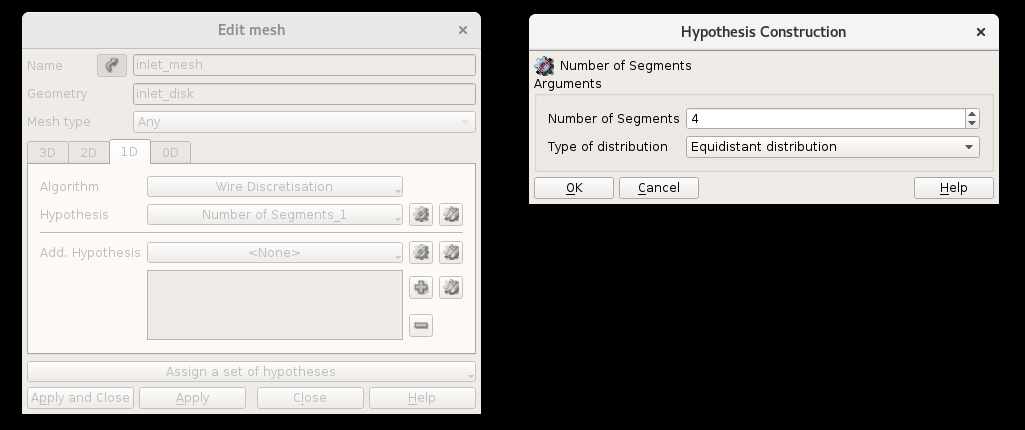
\includegraphics[width =\textwidth]{\IMAGES/3d_mesh.png}
	\caption{Create Mesh}
	\label{lag:mesh_01}
\end{figure}
%
Apply.

In order to prepare the extrusion of the inlet disk, the best way is to mesh two lines following the z-axis and extrude the cylinder along these two lines. The refinement of the lines mesh will be the final refinement of the cylinder in the z-direction. Refinement are set as follows:

Mesh of the first section: 0\_to\_4.0 line
%
\begin{itemize}
	\item \textbf{Name:} 0\_to\_4.0\_mesh
	\item \textbf{Geometry:} 0\_to\_4.0
	\item \textbf{Mesh type:} Any
	\item \menu{1D > Algorithm:} ``Wire Discretisation''
	\item \menu{1D > Hypothesis > Number of segments}: 100 and ``Scale distribution'' with a scale factor of 0.045
\end{itemize}
%
Apply.

Mesh of the second section:
%
\begin{itemize}
	\item \textbf{Name:} 4.0\_to\_5.9\_mesh
	\item \textbf{Geometry:} 4.0\_to\_5.9
	\item \textbf{Mesh type:} Any
	\item \menu{1D > Algorithm:} ``Wire Discretisation''
	\item \menu{1D > Hypothesis > Number of segments} 422 and ``Equidistant distribution''
\end{itemize}
%
Apply.

Then create a mesh group lying on the ``wall'' group created in \geom, by right clicking in the object browser on inlet\_mesh
and selecting \menu{Create Groups from Geometry}. Add the geometry group ``wall'' to the Elements list (\figurename~\ref{lag:ext_wall}).
%
\begin{figure}[H]
	\centering
	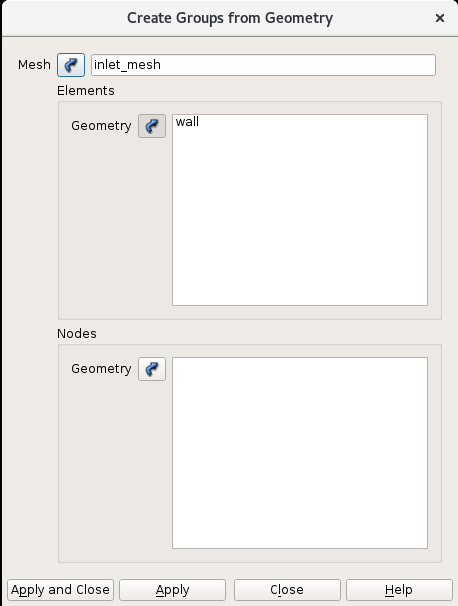
\includegraphics[width = 0.6\textwidth]{\IMAGES/ext_wall.png}
	\caption{Create Groups from Geometry}
	\label{lag:ext_wall}
\end{figure}
%
Compute all meshes (inlet\_mesh, 0\_to\_4.0\_mesh and 4.0\_to\_5.9\_mesh) by right clicking on each mesh and selecting \menu{Compute}.
%
\subsection{Creating Groups in \smesh}
%
Right click on inlet\_mesh and \textbf{Create Group}
%
\begin{itemize}
	\item \textbf{Mesh:} inlet\_mesh
	\item \textbf{Elements Type:} Face
	\item \textbf{Name:} inlet
	\item \textbf{Content:} Select all
\end{itemize}
%
Apply and close.

Now the disk is well discretized and just needs to be extruded along each z-section.

For the first section, select \menu{Modification > Extrusion along a path} and fill the pop-up window as follows:
%
\begin{figure}[H]
	\centering
	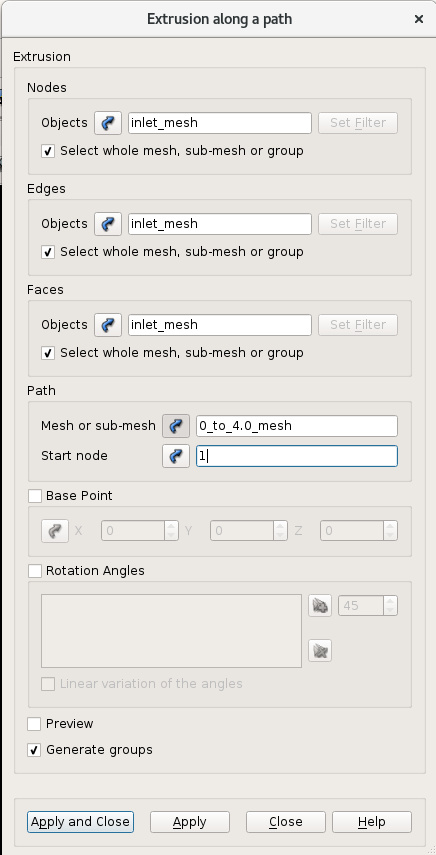
\includegraphics[scale = 0.5]{\IMAGES/extr_1.png}
	\caption{Extrusion along 0\_to\_4.0\_mesh}
	\label{lag:extr_1}
\end{figure}
%
Apply and close.

In Groups of Faces, rename inlet\_top as injection\_plane.

We then need to create a group of cells in which particles will be injected at each iteration of the lagrangian computation.
For this, right click on inlet\_mesh, and select \menu{Create group}. Fill the pop-up window with following settings:
%
\begin{itemize}
	\item \textbf{Mesh:} inlet\_mesh
	\item \textbf{Elements Type:} Volume
	\item \textbf{Name:} injection
	\item \textbf{Group type:} Standalone group
	\item \textbf{Enable manual edition:} toggled
\end{itemize}
%
And select manually the cells around the pipe axis at the injection plane as shown on \figurename~\ref{lag:injection_volume}:
%
\begin{figure}[H]
	\centering
	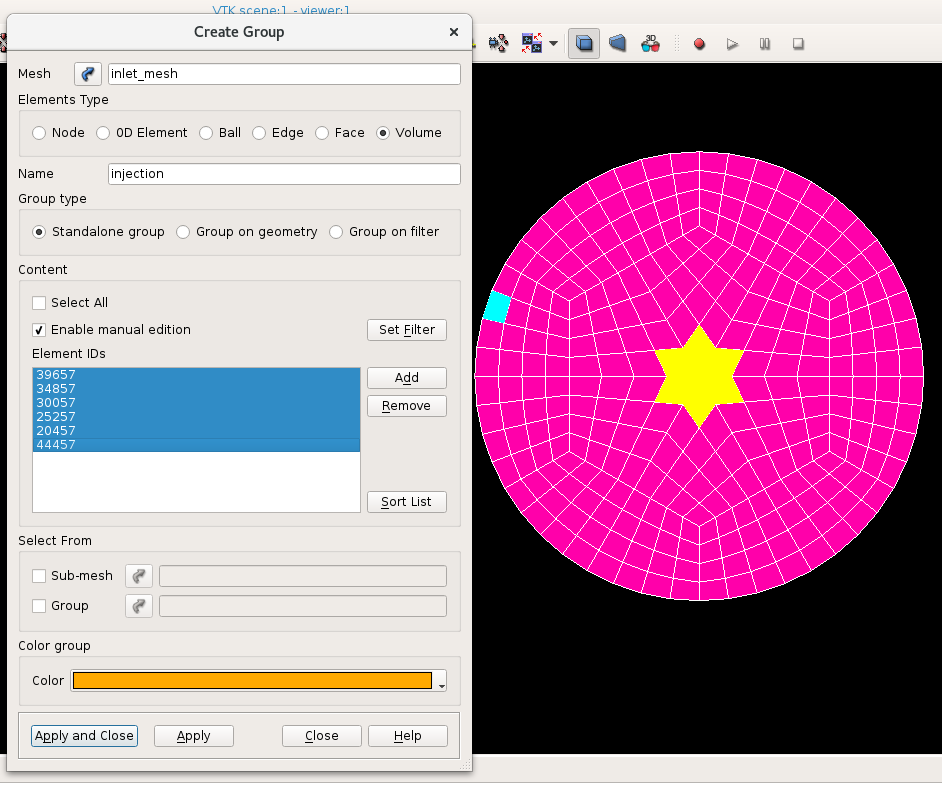
\includegraphics[width=0.8\textwidth]{\IMAGES/injection_group_creation.png}
	\caption{Creation of the injection group}
	\label{lag:injection_volume}
\end{figure}
%
Finally, select the group injection\_plane, created above, and extrude it along 4.0\_to\_5.9.mesh (\figurename~\ref{lag:extr_2}):
%
\begin{figure}[H]
	\centering
	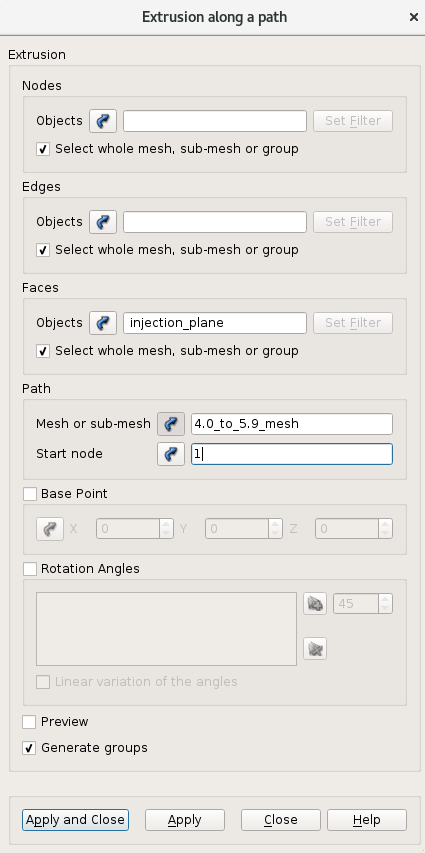
\includegraphics[scale = 0.5]{\IMAGES/extr_2.png}
	\caption{Extrusion along 4.0\_to\_5.9\_mesh}
	\label{lag:extr_2}
\end{figure}
%

Remove all groups of Groups of Edges. In Groups of Faces, select wall\_extruded and wall\_top\_extruded (with \keys{Ctrl}) , click on \menu{Mesh > Union groups} and name it wall.
Apply and close, then remove wall\_top\_extruded and wall\_extruded.
Rename also injection\_plane\_top as outlet. Finally, remove all groups of Groups of Volumes, except, of course, injection. You can also change the groups colors to be able to distinguish them clearly.
%
\clearpage
%
You should get a final mesh as shown on \figurename~\ref{lag:final}.
%
\begin{figure}[H]
	\centering
	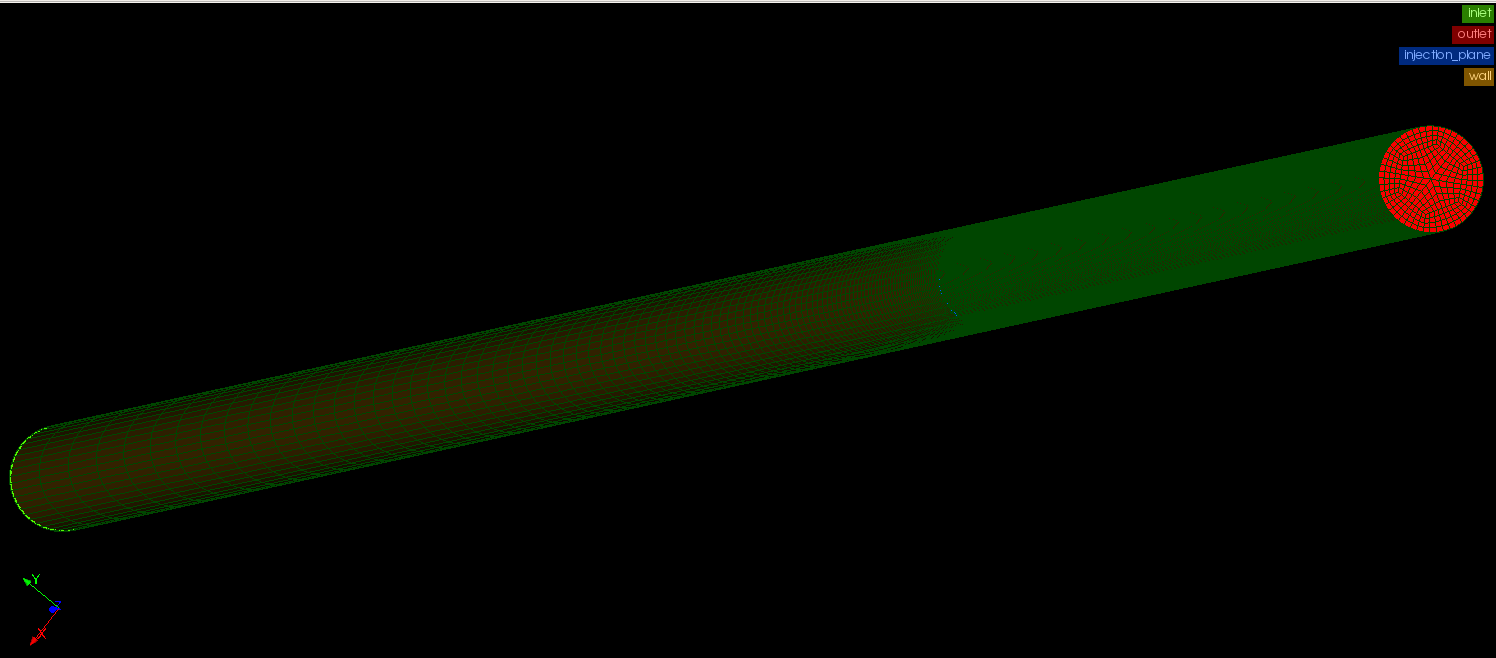
\includegraphics[width = \linewidth]{\IMAGES/final_pipe_mesh.png}
	\caption{volume mesh}
	\label{lag:final}
\end{figure}
%

Two last transformations will be applied to the mesh.

Select \menu{Modification > transformation > Symmetry}.
Toggle \keys{Select whole mesh, sub-mesh or group} and select inlet\_mesh as Name in Arguments.
Apply and close.

Select \menu{Modification > transformation > Translation} and fill the pop-up window as follows (\figurename~\ref{lag:translate}):
%
\begin{figure}[H]
	\centering
	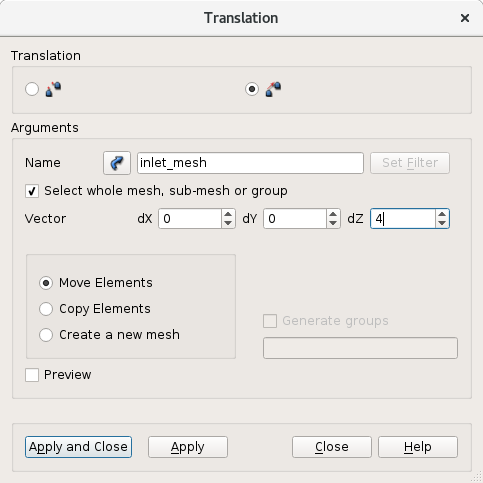
\includegraphics[width=0.7\textwidth]{\IMAGES/translate_mesh.png}
	\caption{Translation of mesh}
	\label{lag:translate}
\end{figure}
%
Apply and Close.

The generation of the computational domain is now completed. Save the \salome file and export the mesh file in ‘.med’ format by selecting from the main menu: \menu{File > Export > MED file}. For the file name, choose ‘Mesh\_ARNASON’; the ‘.med’ extension is automatically added.  You are now ready to move to the CFDStudy module in order to set up the CFD simulation.
